\documentclass[a4paper, oneside, titlepage, reqno]{book}

% pacchetti fondamentali per qualsiasi documento
\usepackage[T1]{fontenc}
\usepackage[utf8]{inputenc}
\usepackage[italian]{babel}
\usepackage[babel, italian=guillemets]{csquotes}
\usepackage[style=numeric]{biblatex}
\usepackage{microtype}


\usepackage{graphicx} % inserire immagini
\usepackage{multicol} % due colonne
\usepackage{ulem} % sottolineare
\usepackage{lipsum} % lorem ipsum
\usepackage{xcolor} % colori in latex

\usepackage[hang]{footmisc} %per le note a pié pagina
\footnotemargin=0.8em

%definizioni particolari
\newcommand{\straniero}[1]{\textit{#1}} %parole straniere
\newcommand{\titolo}[1]{\textsc{#1}} %titoli
% pacchetti matematica
\usepackage[leqno,intlimits]{amsmath} 
\usepackage{amssymb}
\usepackage{amsthm}
\usepackage{yhmath}

\usepackage{pgfplots} % stampare le funzioni
	\pgfplotsset{/pgf/number format/use comma,compat=newest}

\usepackage{cancel} % semplificare

\usepackage{polynom} %divisione tra polinomi

\usepackage{forest} % grafi ad albero

\usepackage{booktabs} % tabelle

% definizione comandi matematici

\DeclareMathOperator{\arcsec}{arcsec}
\DeclareMathOperator{\arccot}{arccot}
\DeclareMathOperator{\arccsc}{arccsc}
\newcommand{\R}{\mathbb{R}}
%rimuovere il titolo del capitolo & impaginazione titolo capitolo
\usepackage{ifthen}
\makeatletter
\def\@makechapterhead#1{%
  \vspace*{30\p@}%
  {\parindent \z@ \raggedright \normalfont
    \vskip 20\p@
    \interlinepenalty\@M
    \Huge \bfseries #1\par\nobreak
    \vskip 40\p@
  }\thispagestyle{fancy}}
\makeatother
\addto\captionsitalian{\renewcommand{\chaptername}{}}
%rimuovere header e footer dalle pagine vuote
\usepackage{ifthen}
\makeatletter
\def\cleardoublepage{\clearpage\if@twoside \ifodd\c@page\else
    \hbox{}
    \vspace*{\fill}
    \vspace{\fill}
    \thispagestyle{empty}
    \newpage
    \if@twocolumn\hbox{}\newpage\fi\fi\fi}
\makeatother
% Creazione dell'ambiente ''NOTA'' 

\usepackage{ifthen}
\usepackage[most]{tcolorbox}
\usepackage{framed}

		\newlength\sidebar
		\newlength\envrule
		\newlength\envborder
		\setlength\sidebar{1.5mm}
		\setlength\envrule{0.4pt}
		\setlength\envborder{2.5mm}
		
		\makeatletter
		\long\def\fboxs#1{%
		  \leavevmode
		  \setbox\@tempboxa\hbox{%
		    \color@begingroup
		      \kern\fboxsep{#1}\kern\fboxsep
		    \color@endgroup}%
		  \@frames@x\relax}
		\def\frameboxs{%
		  \@ifnextchar(%)
		    \@framepicbox{\@ifnextchar[\@frameboxs\fboxs}}
		\def\@frameboxs[#1]{%
		  \@ifnextchar[%]
		    {\@iframeboxs[#1]}%
		    {\@iframeboxs[#1][c]}}
		\long\def\@iframeboxs[#1][#2]#3{%
		  \leavevmode
		  \@begin@tempboxa\hbox{#3}%
		    \setlength\@tempdima{#1}%
		    \setbox\@tempboxa\hb@xt@\@tempdima
		         {\kern\fboxsep\csname bm@#2\endcsname\kern\fboxsep}%
		    \@frames@x{\kern-\fboxrule}%
		  \@end@tempboxa}
		\def\@frames@x#1{%
		  \@tempdima\fboxrule
		  \advance\@tempdima\fboxsep
		  \advance\@tempdima\dp\@tempboxa
		  \hbox{%
		    \lower\@tempdima\hbox{%
		      \vbox{%
		        %\hrule\@height\fboxrule
		        \hbox{%
		         \vrule\@width\fboxrule
		          #1%
		          \vbox{%
		            \vskip\fboxsep
		            \box\@tempboxa
		            \vskip\fboxsep}%
		          #1%
		          }%\vrule\@width\fboxrule}%
		        }%\hrule\@height\fboxrule}%
		                          }%
		        }%
		}
		\def\esefcolorbox#1#{\esecolor@fbox{#1}}
		\def\esecolor@fbox#1#2#3{%
		  \color@b@x{\fboxsep\z@\color#1{#2}\fboxs}{\color#1{#3}}}
		\makeatother
		
		\definecolor{exampleborder}{rgb}{0.5, 0.5, 0.5}
		\definecolor{examplebg}{rgb}{0.89, 0.89, 0.89}
		\definecolor{statementborder}{rgb}{.9,0,0}
		\definecolor{statementbg}{rgb}{1,.9,.9}
		
		\newenvironment{eseframed}{%
		  \def\FrameCommand{\fboxrule=\the\sidebar  \fboxsep=\the\envborder%
		  \esefcolorbox{exampleborder}{examplebg}}%
		  \MakeFramed{\FrameRestore}}%
		 {\endMakeFramed}
		
		\newenvironment{nota}[1]
		{\par\medskip%\refstepcounter{esempio}%
		\hbox{%
		\fboxsep=\the\sidebar\hspace{-\envborder}\hspace{-.5\sidebar}%
		\colorbox{exampleborder}{%
		\hspace{\envborder}\footnotesize\sffamily\bfseries%
		\textcolor{white}{{{\large
		#1}}\hspace{\envborder}}
		}
		}
		\nointerlineskip\vspace{-\topsep}%
		\begin{eseframed}\noindent\ignorespaces%
		}
		{\end{eseframed}\vspace{-\baselineskip}\medskip}
% Comandi per la creazione del riquadro attorno alle equazioni
% \equazione{arg1} crea una equazione con riquadro colorato

\usepackage[leqno,fleqn,intlimits]{empheq}
\usepackage[most]{tcolorbox}
\usepackage{ifthen}

	\newif\ifmarg
	\margtrue
	\ifmarg
	\makeatletter
	\let\mytagform@=\tagform@
	\def\tagform@#1{\maketag@@@{\mbox{~}\hbox{\rlap{\hspace{0.5in}(\ignorespaces#1\unskip\@@italiccorr)}}}\kern1sp}
	\renewcommand{\eqref}[1]{{\mytagform@{\ref{#1}}}}
	\makeatother
	\fi
	
	\newcommand*\mygraybox[0]{%
		\tcbhighmath}
		
	\newcommand{\equazione}[1]{	\begin{empheq}[box=\mygraybox]{equation*}
			#1
		\end{empheq}}

\usepackage{geometry}
\geometry{top=5.5cm, left=125pt, right=125pt,%
heightrounded}
\usepackage{fancyhdr}
\pagestyle{fancy}
\usepackage{calc}
\newlength{\oddmarginwidth}
\setlength{\oddmarginwidth}{15mm+\hoffset+\oddsidemargin}
\newlength{\evenmarginwidth}
\setlength{\evenmarginwidth}{\evensidemargin+15mm}
\fancyhfoffset[LO,RE]{\oddmarginwidth}
\fancyhfoffset[LE,RO]{\evenmarginwidth}
\renewcommand{\headrulewidth}{0.5pt}
\renewcommand{\footrulewidth}{0.5pt}
\fancyhead[L]{\hspace{2em}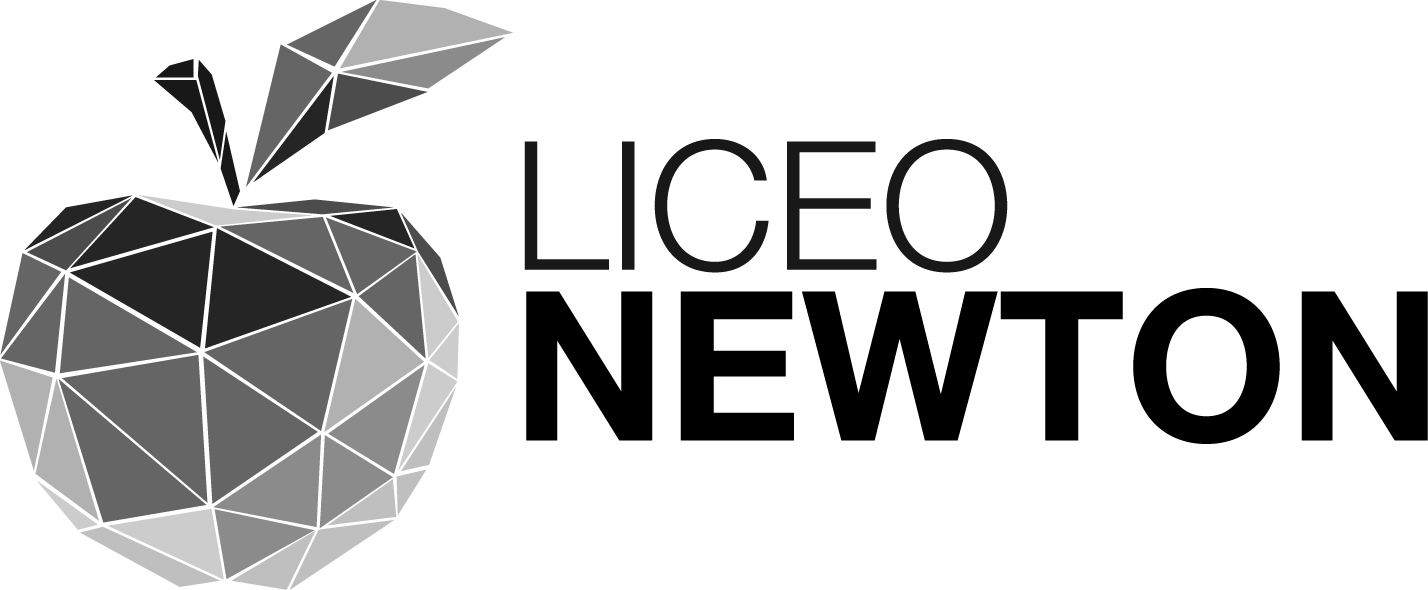
\includegraphics[width=4cm]{1}\vspace{1.4cm}}
\fancyhead[R]{
\includegraphics[width=1.5cm]{2}\hspace{2em}\vspace{1.4cm}}
\fancyhead[C]{{\Large Liceo Classico Scientifico Musicale ``\textbf{Isaac Newton}''}\\ \vspace{0.3em}%
{\large via Paleologi 22, Chivasso (TO)}\vspace{1em}}
\fancyfoot[C]{\thepage}
\fancyfoot[R]{\textbf{Elaborati Esame di Stato 20-21}}
\geometry{top=5.5cm, left=125pt, right=125pt, headsep=11.47mm, headheight=32.82mm, footskip=23.73mm,%
heightrounded}

\bibliography{biblio}

\addtolength{\skip\footins}{2em} % aumentare spazio prima di footnotes

%-----------


% comandi particolari per questo documento

\newcommand{\kappaa}{k}
\newcommand{\aaaa}{a}

\renewcommand\arraystretch{1.3}  %altezza righe tabella

\renewcommand{\theequation}{\arabic{equation}}

\renewcommand{\thefootnote}{\alph{footnote}}

\newcommand{\red}[1]{\textcolor{red}{#1}}

%----------

\usepackage{layout}

% Hyperref

\usepackage{hyperref}
            
\hypersetup{%
	pdfauthor={Davide Peccioli},
	pdftitle={Analisi numerica e applicazioni},
	pdfsubject={Matematica e fisica},
	allcolors=blue, 
	colorlinks=true}
	
%------------

\begin{document}

\begin{titlepage} % pagina del titolo
\thispagestyle{fancy}
\begin{center}
    \null
    \vfill
    {\huge Analisi numerica e applicazioni}\\
    \vspace{3em}
    {\large Davide Peccioli}\\
    \vspace{1em}
    {\large \textbf{Classe 5\textsuperscript{a}\,H}}
    \fancyfoot[C]{}
    \vfill
\end{center}
\end{titlepage}

\fancyfoot[C]{\thepage}

\tableofcontents\thispagestyle{fancy}

\chapter{Analisi numerica e applicazioni}

\begin{nota}{Consegna}
L’analisi numerica si occupa della ricerca delle procedure di calcolo per la determinazione di soluzioni approssimate di problemi ambientati in un insieme numerico continuo.

Il candidato esponga le principali metodologie utilizzate in un ambito scelto (ricerca soluzioni di equazioni, integrazione, etc.) e, in particolare, è richiesto di:

\begin{enumerate}
\item studiare una funzione del tipo $y=x^5+kx+1$, avendo scelto un parametro $k$ ($k<2$), commentando in modo puntuale gli aspetti teorici utilizzati;
\item fornire indicazioni per lo sviluppo di un algoritmo che permetta di individuare gli zeri della funzione scelta;
\item esporre un’applicazioni matematica o fisica (es. calcolo aree, interpolazioni…).
\item Una forza $\vec{F}$ nella direzione dell’asse $x$ agisce su un oggetto in moto lungo l’asse $x$. Se l’intensità della forza è data da $F=10e^{-x/2,0}\,\text{N}$ trovare il lavoro svolto da $\vec{F}$ mentre l’oggetto si sposta da $x=0$ a 
$x= 2,0\,\text{m}$ 
\begin{enumerate}
\item tracciando la curva F(x) e valutando per via grafica l’area sottesa dalla curva e
\item per via analitica, calcolando l’integrale.
\end{enumerate}
\end{enumerate}
\end{nota}

\chapter{Studio di funzione}

Si studi la funzione 

\begin{equation}
y=f(x)=x^5+kx+1
\end{equation}

\section{Scelta del parametro}

Prima di studiare la funzione in questione è necessario assegnare al parametro $k$ un valore reale ($k<2$), tale per cui  la funzione presenti uno zero doppio. Questa scelta è dettata dalle considerazioni che si possono fare proprio in merito a tale punto.

Utilizzando il \textbf{teorema fondamentale dell'algebra}\supercite{courant:mate}, posso scrivere il polinomio $f(x)$ come:
\[
f(x)=(x-\alpha)\cdot(x-\beta)\cdot(x-\gamma)\cdot(x-\delta)\cdot(x-\varepsilon)
\]
dove $\alpha$, $\beta$, $\gamma$, $\delta$, $\varepsilon$ sono le radici, reali o complesse, del polinomio.

Dal momento che si ricerca un polinomio con uno zero doppio, possiamo scrivere:
\begin{multline*}
f(x)=\\
=(x-\alpha)^2\cdot(x-\beta)\cdot(x-\gamma)\cdot(x-\delta))=\\
=(x-\alpha)^2\cdot p(x)
\end{multline*}
da cui
\[
p(x)=\frac{f(x)}{(x-\alpha)^2}
\]

Per il \textbf{teorema di Ruffini}\supercite{blu:1} posso quindi affermare che la divisione $\frac{f(x)}{(x-\alpha)^2}$ non deve avere resto\footnote{Il teorema di Ruffini afferma che
\begin{quotation}
Un polinomio $P(X)$ è divisibile per $(x-a)$ \textit{se e solo se} $P(a)=0$.
\end{quotation}
Dal momento che per ipotesi $\alpha$ è radice doppia del polinomio, $f(x)$ è divisibile doppiamente per $(x-\alpha)$}. Questa sarà proprio la condizione che permetterà di trovare un valore di $k$ adeguato.
Espandendo $(x-\alpha)^2$ come $x^2-2\alpha x+\alpha^2$ si svolge la divisione polinomiale:
\[
\begin{array}{cccccc|c}
x^5 & +0x^4 & +0x^3 & +0x^2 & +kx & +1  & x^2-2\alpha x+\alpha^2\\ \cline{7-7}
x^5 & -2\alpha x^4 & +\alpha^2x^3 & & & & x^3+2\alpha x^2+3\alpha^2x+4\alpha^3\\\cline{1-3}
& 2\alpha x^4 & -\alpha^2x^3 & & & & \\
& 2\alpha x^4 & -4\alpha^2x^3 & +2\alpha^3x^2 & & & \\
\cline{2-4}
& & 3\alpha^2x^3 & -2\alpha^3x^2 &+ kx & & \\
& & 3\alpha^2x^3 & +6\alpha^3x^2 & +3\alpha^4x & & \\
\cline{3-5}
& & & 4\alpha^3x^2 & (k-3\alpha^4)x & + 1& \\
& & & 4\alpha^3x^2 & -8\alpha^4x & +4\alpha^5 & \\
\cline{4-6}
& & & & (k+5\alpha^4)x & -4\alpha^5 + 1& 
\end{array}
\]
Il cui resto $r(x)$ è
\[
r(x)=(k+5\alpha^4)x -4\alpha^5 + 1
\]

Per le condizioni esposte precedentemente
\[
r(x)=0\quad \forall x\in \R
\]
da cui
\[
\begin{cases}
k+5\alpha^4=0\\
-4\alpha^5+1=0
\end{cases}
\]

Le soluzioni di questo sistema sono
\[
\alpha=\sqrt[5]{\frac{1}{4}}
\]
\equazione{k=-\frac{5}{2\sqrt[5]{8}}}
La funzione da studiare diventa quindi
\begin{equation}
y=f(x)=x^5-\frac{5}{2\sqrt[5]{8}}\cdot x+1
\end{equation}

\section{Studio di funzione}

\subsubsection*{Campo di esistenza}

Come per tutte le funzioni polinomiali, il campo di esistenza della funzione è 
\[
x\in\R
\]

\subsubsection*{Limiti}

\begin{gather*}
\lim_{x\to+\infty}\Big(x^5-\frac{5}{2\sqrt[5]{8}}\cdot x+1\Big)=+\infty\\
\lim_{x\to-\infty}\Big(x^5-\frac{5}{2\sqrt[5]{8}}\cdot x+1\Big)=-\infty
\end{gather*}

Essendo una funzione polinomiale, sicuramente non presenta asintoti obliqui.

\subsubsection*{Zeri}

Abbiamo definito in precedenza $f(x)=(x-\alpha)^2\cdot (x^3+2\alpha x^2+3\alpha^2x+4\alpha^3)$, con $\alpha=\sqrt[5]{\frac{1}{4}}$. Pertanto
\[
f(x)=0\,\iff\, (x-\alpha)=0\,\lor\,(x^3+2\alpha x^2+3\alpha^2x+4\alpha^3)=0
\]
La prima equazione:
\[x-\alpha=0\,\implies\, x=\alpha\]
\equazione{x=\sqrt[5]{\frac{1}{4}}}
La seconda è una equazione di terzo grado\supercite{eq:ter}:
\begin{gather*}
\textcolor{red}{27\times\,\Bigg(}x^3+2\alpha x^2+3\alpha^2x+4\alpha^3=0\textcolor{red}{\Bigg)}\\
27x^3+54\alpha x^2+81\alpha^2 x + 108 \alpha^3=0
\end{gather*}
Sia \red{$t=3x+2\alpha$}, da cui $x=(t-2\alpha)/3$
\begin{gather*}
27\Big(\red{\frac{t-2\alpha}{3}}\Big)^3+54\alpha \Big(\red{\frac{t-2\alpha}{3}}\Big)^2+81\alpha^2 \Big(\red{\frac{t-2\alpha}{3}}\Big) + 108 \alpha^3=0\\
\dots\\
t^3+(27\alpha^2-12\alpha^2)t+108\alpha^3-54\alpha^3+16\alpha^3=0\\
t^3+15\alpha^2t+70\alpha^3=0
\end{gather*}
Si cerca $t$ nella forma $t=u+v$
\[
(u+v)^3+15\alpha^2(u+v)+70\alpha^3=0
\]
\begin{multline*}
u^3+v^3-3u^2v+3uv^2+15\alpha^2(u+v)+70\alpha^3=\\
=u^3+v^3+3uv(u+v)+15\alpha^2(u+v)+70\alpha^3=\\
=u^3+v^3+(3uv+15\alpha^2)(u+v)+70\alpha^3=0
\end{multline*}

Siccome esistono tanti modi per scrivere $t$ come $t=u+v$ è possibile imporre un'ulteriore condizione. Per semplicità di calcolo, sia
\[
3uv+15\alpha^2=0
\]
da cui
\[
\begin{cases}
u^3+v^3=-70\alpha^3\\
3uv=-15\alpha^2
\end{cases}
\implies\begin{cases}
u^3+v^3=-70\alpha^3\\
27u^3v^3=-3375\alpha^6
\end{cases}
\]
Siano $s_1=u^3$ e $s_2=v^3$
\[
\begin{cases}
s_1+s_2=-70\alpha^3\\
s_1\cdot s_2=-125\alpha^6
\end{cases}
\]
Risolvere questo sistema significa risolvere l'equazione di secondo grado
\begin{gather*}
s^2+(70\alpha^3)\,s-125\alpha^5=0\\
s_{1,2}=-\frac{70\alpha^3}{2}\pm\sqrt{\frac{4900\alpha^6}{4}+125\alpha^6}\\
s_{1,2}=-35\alpha^3\pm\sqrt{1350\alpha^6}\\
\begin{cases}
s_1=(-35+15\sqrt{6})\alpha^3\\
s_2=-(35+15\sqrt{6})\alpha^3
\end{cases}
\end{gather*}

Riprendendo le equazioni precedenti
\begin{multline*}
t=u+v=\\
=\sqrt[3]{s_1}+\sqrt[3]{s_2}=\alpha\sqrt[3]{-35+15\sqrt{6}}-\alpha\sqrt[3]{35+15\sqrt{6}}=\\
\alpha\Bigg[\sqrt[3]{-35+15\sqrt{6}}-\sqrt[3]{35+15\sqrt{6}}\Bigg]
\end{multline*}
da cui, dato che $x=t/3-2a/3$:
\begin{multline*}
x=\frac{\alpha}{3}\cdot\Bigg[\sqrt[3]{-35+15\sqrt{6}}-\sqrt[3]{35+15\sqrt{6}}-2\Bigg]=\\
=\frac{\sqrt[3]{-35+15\sqrt{6}}-\sqrt[3]{35+15\sqrt{6}}-2}{3\sqrt[5]{4}}\approx\\
\approx -1,2509430053151
\end{multline*}
\equazione{x\approx -1,2509430053151}
Sia questo numero $\beta$.

\subsubsection*{Segno}
\[
y=(x-\alpha)^2\cdot p(x)
\]

$p(x)$ è un polinomio di terzo grado, con un'unica intersezione con l'asse delle $x$ (in $x=\beta$, vedasi dimostrazione precedente). Essendo una funzione continua e derivabile $\forall x\in\R$, è possibile affermare che tutte le immagini dei punti nell'intervallo $(-\infty; \,\beta)$ avranno segno concorde; allo stesso modo per le immagini dei punti nell'intervallo $(\beta; \,+\infty)$\footnote{Ragionando per assurdo, si ammetta che nell'intervallo $(-\infty; \,\beta)$ esistano due punti la cui immagine abbia segno discorde. Siano questi punti $a$ e $b$. Si consideri l'intervallo $[a;\,b]$: è possibile applicare il \textbf{teorema dell'esistenza degli zeri}, che afferma che nell'intervallo considerato esiste almeno uno zero. Questo va contro l'ipotesi iniziale che $\beta$ sia l'unico zero della funzione. Si ragioni allo stesso modo per l'intervallo $(\beta; \,+\infty)$.}.

Considerato che $(x-\alpha)^2>0\,\forall x\in \R-\{\alpha\}$, la funzione $p(x)$ sarà avrà segno concorde a $f(x)\,\forall x\in \R-\{\alpha\}$. Per $x=\alpha$, essendo $\alpha\neq\beta$ e $\alpha>\beta$, $p(\alpha)$ avrà lo stesso segno di tutti gli altri punti nell'intervallo $(\beta; \,+\infty)$. Pertanto:
\[
\lim_{x\to-\infty}f(x)=-\infty\,\implies\,\lim_{x\to-\infty}p(x)<0\implies p(x)<0\,\forall x\in (-\infty;\,\beta)
\]
\[
\lim_{x\to+\infty}f(x)=+\infty\,\implies\,\lim_{x\to-\infty}p(x)>0\implies p(x)>0\,\forall x\in(\beta; \,+\infty)
\]

È possibile ora studiare il segno della funzione $y=f(x)$:
\begin{center}
\begin{tikzpicture}
%\draw [help lines] (0,0) grid (9,3);
\draw [thick, ->] (0,2.5) -- (9,2.5);
\draw [teal, ultra thick] (0,1.9) -- (9,1.9);
\draw [cyan, ultra thick] (3.5,1.4) -- (9,1.4);
\draw [cyan, ultra thick, dashed] (0,1.4) -- (3.5,1.4);
\draw (3.5,2.4) -- (3.5,2.6);
\draw (5.5,2.4) -- (5.5,2.6);
\node at (3.5, 2.8) {$\beta$};
\node at (5.5, 2.8) {$\alpha$};
\node at (-0.7,1.9) {$\textcolor{teal}{(x-\alpha)^2}$};
\node at (9.7,1.4) {$\textcolor{cyan}{p(x)}$};
\draw [dashed] (3.5, 0.5) -- (3.5, 2.5);
\draw [dashed] (5.5, 0.5) -- (5.5, 2.5);
\node [draw, circle, inner sep=2pt, fill=white] at (3.5,1.4) {};
\node [draw, circle, inner sep=2pt, fill=white] at (3.5,0.5) {};
\node [draw, circle, inner sep=2pt, fill=white] at (5.5,1.9) {};
\node [draw, circle, inner sep=2pt, fill=white] at (5.5,0.5) {};
\draw [ultra thick] (1.7,0.5) -- (2,0.5);
\draw [ultra thick] (4.35,0.5) -- (4.65,0.5);
\draw [ultra thick] (7.35,0.5) -- (7.65,0.5);
\draw [ultra thick] (4.5,0.35) -- (4.5,0.65);
\draw [ultra thick] (7.5,0.35) -- (7.5,0.65);
\node at (0.5,0.5) {$f(x)$};
\end{tikzpicture}
\end{center}

\equazione{f(x)>0\quad\forall x\in (\beta;\,\alpha)\,\cup\,(\alpha;\,+\infty)}

\subsubsection*{Derivata prima}
\[
y'=5x^4-\frac{5}{2\sqrt[5]{8}}
\]
Il segno della derivata prima rappresenta se la funzione stia crescendo o decrescendo; quando la derivata prima si annulla la funzione avrà un \textbf{punto stazionario}.

\[
y'=0\,\implies\,x^4=\frac{1}{2\sqrt[5]{8}}\,\implies\,x=\pm\sqrt[4]{\frac{1}{2\sqrt[5]{8}}}=\pm\frac{1}{\sqrt[5]{4}}
\]
Questi sono i punti stazionari della funzione. Studiando il segno della derivata sarà possibile stabilire se siano anche massimi o minimi.

\[
y'>0\,\implies\,5x^4-\frac{5}{2\sqrt[5]{8}}>0\,\implies\,\big(x^2\big)^2>\frac{1}{2\sqrt[5]{8}}
\]
\begin{gather*}
x^2>\sqrt{\frac{1}{2\sqrt[5]{8}}}\\\lor\\x^2<-\sqrt{\frac{1}{2\sqrt[5]{8}}}\quad\text{\textbf{mai}}
\end{gather*}
\[
x^2>\sqrt{\frac{1}{2\sqrt[5]{8}}}\,\implies\,x>\frac{1}{\sqrt[5]{4}}\,\lor\,x<-\frac{1}{\sqrt[5]{4}}
\]

Pertanto
\[
y'>0\quad\forall x\in \Bigg(-\infty;\,-\frac{1}{2\sqrt[5]{8}}\Bigg)\,\cup\,\Bigg(\frac{1}{2\sqrt[5]{8}};\,+\infty\Bigg)
\]
\begin{center}
\begin{tikzpicture}
%\draw [help lines] (0,0) grid (9,3);
\draw [->] (-1,2.5) -- (5,2.5);
\draw [thick] (-1,1.9) -- (1,1.9);
\draw [thick] (3,1.9) -- (5,1.9);
\draw [thick, dashed] (1,1.9) -- (3, 1.9);
\draw (1,2.4) -- (1,2.6);
\draw (3,2.4) -- (3,2.6);
\node at (1, 3) {$-1/(2\sqrt[5]{8})$};
\node at (3, 3) {$1/(2\sqrt[5]{8})$};
\node at (-1.5,1.9) {$y'$};
\draw [dashed] (1, 0) -- (1, 2.5);
\draw [dashed] (3, 0) -- (3, 2.5);
\node [draw, circle, inner sep=2pt, fill=white] at (1,1.9) {};
\node [draw, circle, inner sep=2pt, fill=white] at (3,1.9) {};
\node at (-1.5,0.7) {$f(x)$};
\draw [cyan, ->, ultra thick] (-0.8, 0.3) -- (0.8, 1.5);
\draw [cyan, ->, ultra thick] (3.2, 0.3) -- (4.8, 1.5);
\draw [cyan, ->, ultra thick] (1.2, 1.5) -- (2.8, 0.3);
\node at (1,-0.25) {\textbf{max\vphantom{i}}};
\node at (3,-0.25) {\textbf{min}};
\end{tikzpicture}
\end{center}

Come si può vedere dal grafico sopra riportato, il punto
\[M_1\Bigg(-\frac{1}{2\sqrt[5]{8}};\, 2\Bigg)\]
è punto di \textbf{massimo}, mentre il punto
\[
M_2\Bigg(\frac{1}{2\sqrt[5]{8}};\,0\Bigg)
\]
è punto di \textbf{minimo}, nonché zero della funzione.

\subsubsection*{Derivata seconda}
\[
y''=20x^3
\]

Lo studio del segno della derivata seconda fornisce informazioni sulla concavità di una funzione: quando la derivata seconda è positiva, la concavità della funzione è rivolta verso l'alto, quando la derivata seconda è negativa la concavità della funzione è rivolta verso il basso, e quando la derivata seconda si annulla la funzione ha un \textbf{flesso obliquo}, punto in cui la funzione cambia concavità.

\begin{gather*}
y''=0 \,\iff\, x=0\\
y''>0\quad\forall x\in (0;\,+\infty)\\
y''<0\quad\forall x\in (0;\,+\infty)
\end{gather*}

Ora è possibile disegnare la funzione su un piano cartesiano.

\begin{tikzpicture}
\begin{axis} [xmin=-5,xmax=5, ymin=-5, ymax=5, axis equal, xlabel=$x$, ylabel=$y$, title={Grafico di funzione}, width=\textwidth, axis lines=middle]

\end{axis}
\end{tikzpicture}

\cleardoublepage
\printbibliography\addcontentsline{toc}{chapter}{\bibname}\thispagestyle{fancy}

\end{document}